\section{The Structure of the Solver}

The requirements, in particular the points  \ref{AnfImmed}, \ref{AnfLinear} and
\ref{AnfNonlinear}, set up in  chapter \ref{SolverAnforderungen} and schematically represented the structuring of the equations solvers  in figure \ref{Grobstruktur} suggests to lay down this into five largely independent main modules, see \cite{Trispel}. Built up on this structure and the heuristic algorithms described in the preceding chapter,  the Macsyma program packet \verb+SOLVER+ was developed for the functionality extension of the Macsyma functions \verb+SOLVE+ and \verb+LINSOLVE+.

The tasks of the module {\em Solver Preprocessor} are general, checking the command syntax and semantics, the construction of internal data structures, and the execution of an introductory consistency check. The check determines whether the set of equations directly contains contradictory  statements like  number = number or constraint conditions between parameters .

The {\em Immediate Assignment Solver}  searches the system of equations for direct assignments of the form $\mbox{\em var} = \const$ or $\const = \mbox{\em var}$ before the call of the {\em Linear Solvers}  and executes these immediately, so that the cost of computation  for the following program module is kept as small as possible.

The  {\em Linear Solver} is a pre and post processor for the Maxima function \verb+LINSOLVE+  for the simultaneous solution of linear systems of equations. The module extracts  pieces  of linear equations according to the heuristic algorithm described in paragraph \ref{HeurAlgoLin}  and solves the equations by calling \verb+LINSOLVE+. The resulting solutions are inserted into the remaining equations before leaving the {\em Linear Solvers}.

The {\em Valuation Solver} is the core module of the  {\em Solvers}. Its tasks are the use of valuation strategies for the generation of the solution sequences and the solution of the nonlinear equations with the help of the Maxima build-in function \verb+SOLVE+. In the case of multiple solutions the {\em Valuation Solver}  checks each individual solution for consistency with the remaining system of equations. Inconsistent solutions are rejected, while valid solutions are inserted into the remaining system  of equations and the corresponding solution paths are tracked separately through recursive  calls of the {\em Valuation Solvers}.

All steps necessary for the editing of the solutions for output to the user are taken over  by the {\em Solver Postprocessor}. These are the expansion of the hierarchically organized solution list supplied by the {\em Valuation  Solver}, the back substitution of the
symbolic solutions as well as picking out, evaluating and outputting the variables and composite terms asked for by the user.

\begin {figure} [htbp]
\begin {center}
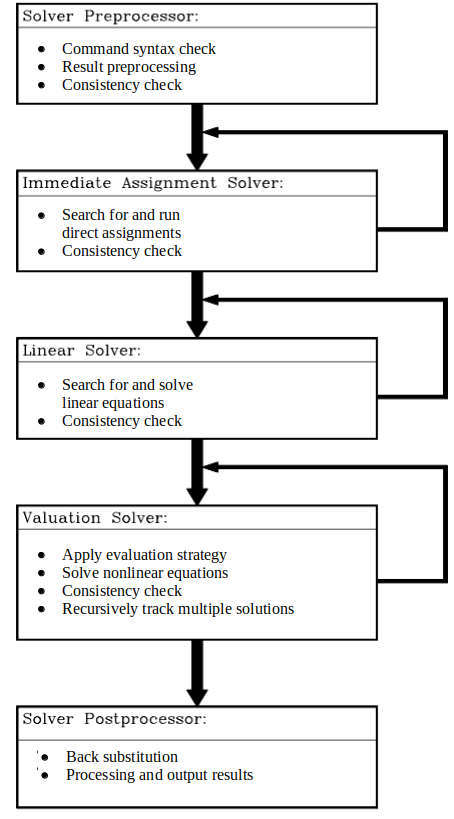
\includegraphics[height=10cm]{StrukturEn.png}
\caption \protect {\begin {minipage} [h] {10cm}% --- TABLE
Structure of the Solvers
\label{Grobstruktur}
\end {minipage}
}
\end {center}
\end {figure}

%\inbildpsf{Struktur des Solvers}{struktur.eps}{100mm}{Grobstruktur}
\clearpage

\section{The Modules of Solvers}

\subsection{The Solver Preprocessor}

\begin {figure} [htbp]
\begin {center}
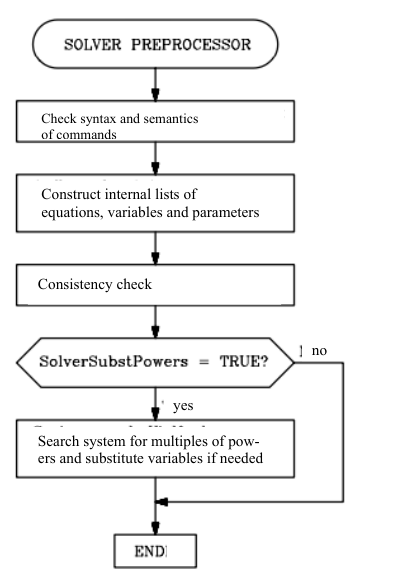
\includegraphics[height=8cm]{PreprocEn.png}
\caption \protect {\begin {minipage} [h] {10cm}% --- TABLE
Flow diagram of the  Solver Preprocessor\label{AblPreproc}
\end {minipage}
}
\end {center}
\end {figure}

%\inbildpsf{Ablaufdiagramm des Solver Preprocessors}{preproc.eps}{60mm}%
%{AblPreproc}

Beside the examination of the command syntax and semantic as well as the construction of the internal equations, variables and parameter lists,  the {\em Solver Preprocessor} executes a consistency check of the equations, whose flow diagram is represented in figure \ref{AblConsChk}. Aim of the consistency check is it to detect from the beginning, whether the system of equations is unsolvable due to direct contradictions. Such contradictions can occur in form of pure number equations, e.g. \ $0=1$, or in addition, in the form of constrained  conditions between symbols declared as parameters.

In order to uncover direct contradictions, the routine for the consistency check searches after equations in the system of equations, which consist exclusively of numbers  or numbers with parameters, but does not contain variables.  If a contradictory number equation is found, then the  {\em Solver Preprocessor}  aborts immediately. If such an equation is  consistently, as for example $0=0$, it is removed from the system of equations, since it does not influence the solubility and solution of the system  and therefore is redundant.

The handling of parameters with constrain conditions is somewhat more complex. Assumed, the symbols $A$ and $B$ were defined as parameters of a system of equations, which contains the equation 
\begin{equation} \label{ParamConstraint}
A + B = 1
\end{equation}

\begin {figure} [htbp]
\begin {center}
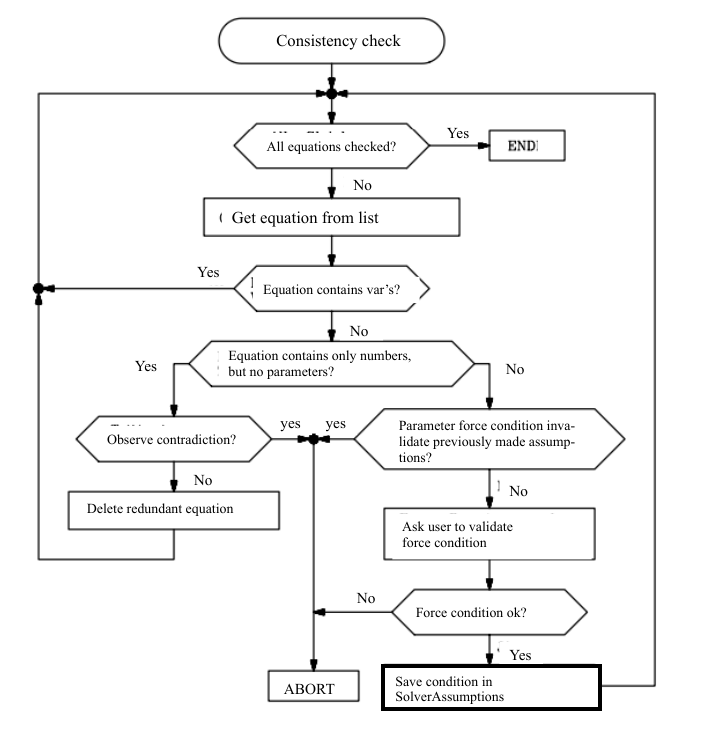
\includegraphics[height=8cm]{ConschkEn.png}
\caption \protect {\begin {minipage} [h] {10cm}% --- TABLE
Flow diagram of the routine for the consistency check\label{AblConsChk}
\end {minipage}
}
\end {center}
\end {figure}

%\inbildpsf{Ablaufdiagramm der Routine zur Konsistenzpr"ufung}{conschk.eps}%
%{125mm}{AblConsChk}

From this condition follows, that $A$ and $B$ are not {\em independent} parameters and therefore the system of equations is not solvable for any combinations of their values. Since conditioned inconsistencies of this type cannot be excluded with many technical problem settings, it is not meaningful to abort the solution process in such cases unless the parameterized equation contradicts  other constraints  in the system of equations. The decision, whether a parameter constraint is to be regarded as admissible, is delegated therefore by the consistency check to the user. In the case of the equation (\ref{ParamConstraint}) the system asks in the following way for the validity of the condition:
\begin{literatim}{|}
Is   B + A - 1   positive, negative, or zero?
\end{literatim}

Becomes the question answered with \verb+p;+ or \verb+n;+ ({\em positive} resp.\ {\em
negative}), then the Solver aborts. If the response reads \verb+z;+ ({\em zero}), then the consistency check stores the constained condition in a global list named \verb+SolverAssumptions+, which can be inspected after the Solver run. Subsequently, the consistency check removes the redundant equation from the system.

% ch 2.2
\subsection{The Immediate Assignment Solver}

\begin {figure} [htbp]
\begin {center}
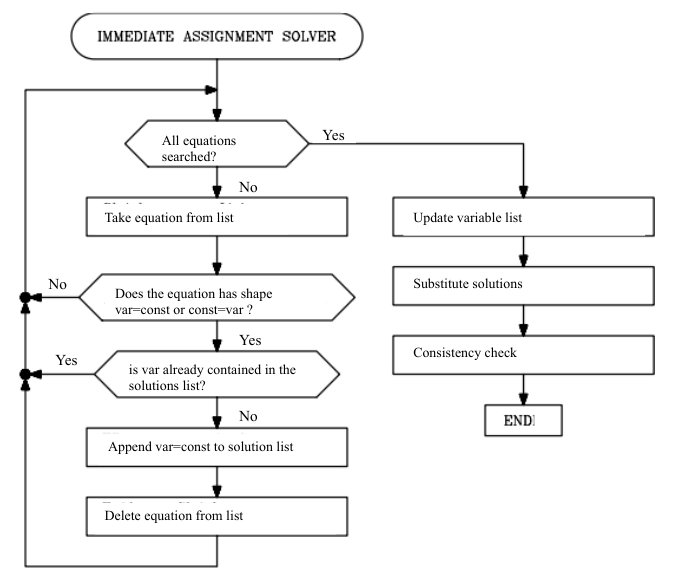
\includegraphics[height=8cm]{ImmedEn.png}
\caption \protect {\begin {minipage} [h] {10cm}% --- TABLE
Flow diagram of the Immediate Assignment Solver\label{AblImmed}
\end {minipage}
}
\end {center}
\end {figure}

%\inbildpsf{Ablaufdiagramm des Immediate Assignment Solvers}{immed.eps}%
%{125mm}{AblImmed}

The task of the {\em Immediate Assignment Solvers} is to search the system of equations for direct assignments of the form $\mbox{\em var} = \const$  and to use such equations directly for the elimination of the corresponding variables. With systems of equations, set up  mechanically, as for instance in the example \ref{ET}, the cost of computation  in  {\em Linear Solver}  for the extraction and solution of the linear equations can be often reduced considerably by such a preprocessing of the equations.

At first, the {\em Immediate Assignment Solvers }  filters out all direct assignments  $\mbox{\em var} = \const$ and $\const = \mbox{\em var}$ from the system  in a loop and stores them in the form $\mbox{\em var} = \const$ in the solution list, if a solution for {\em var}  is not yet entered. Subsequently, the system of equations is analyzed by means of the solution list  and checked again for consistency.

\clearpage

\subsection{The Linear Solver}% 2.2.3

The process of the {\em Linear Solvers} starts, as described in paragraph \ref{HeurAlgoLin}, with the construction of the complete coefficient matrix of the symbolic system of equations. Using this coefficient matrix, the valuation matrix is created, which serves for the extraction of  parts of linear equations. As long as the valuation matrix contains still '1' elements, i.e. $\sum C \neq 0$ und $\sum R \neq 0$, the described heuristic evaluation strategy  is applied, which decides, which nonlinear equation is removed or which in a nonlinear sense occurring variable is transferred to right hand side of the equation.

If the valuation matrix was reduced to a zero-matrix, then a list of the remaining (linear) equations and a list of the linear variables are created, which can be transferred as function parameters to the Maxima instruction \verb+LINSOLVE+, which  serves for the solution of a linear system of equations. 
For efficiency,  before the call of \verb+LINSOLVE+ however, still another special feature is considered, which was not mentioned during the description of the extraction algorithm. Occasionally it can occur, that simultaneously with the deleting of a nonlinear equation the only instance of a linear variable $x_j$ is removed  from the entire valuation matrix, without that it was noticed directly. 
Likewise equations can develop, which are no longer nonlinear w.r.t as linear detected variables, but do not contain these variables any more, i.e. the associated coefficients are directly zero. 
Therefore,  all linear variables of the linear subsystem are  again checked, whether they are still contained in the linear equations, an
The {\em Linear Solver}
would also be able to solve the system of equations without these additional measures, but frequently unnecessary cost of computation can be saved by it.

In section \ref{LoesungLin}, it was demonstrated, that while solving of over-determined linear systems of equations, inconsistencies can occur, which does not necessarily imply the insolubility of the system of equations. If such contradictory equations are detected, e.g. the right side of equation  (\ref{constraint})\footnote{That access to the contradictory equations from the outside is not possible using the standard  {\tt LINSOLVE} command.  Therefore a particularly modified version of the instruction  on Lisp level was necessary, which was made available by Jeffrey P.\ Golden, Macsyma, Inc. (the USA), on a kindly request.}, 
they are submitted a consistency checking, as at the beginning the entire system of equations. If the contradictory equations prove as true inconsistencies, then the total system does not have a solution, and the {\em Linear Solver} aborts with an appropriate error message. If the contradictory equations contain still looked-for variables, then they are removed from the system of equations and added as new constrained  conditions to the remaining system. Thereupon \verb+LINSOLVE+ is again called  with the linear independent part of the equations (inconsistencies can not occur any longer with the second run).

If the linear equations were successfully solved, then the solutions are inserted into the remaining system of equations and the list of the looked-for variables is updated. That is, all variables, for which a solution was found  by the {\em Linear Solver}, are removed from the list, while new variables, which are contained in these solutions, are added to the list.

\clearpage

\begin {figure} [htbp]
\begin {center}
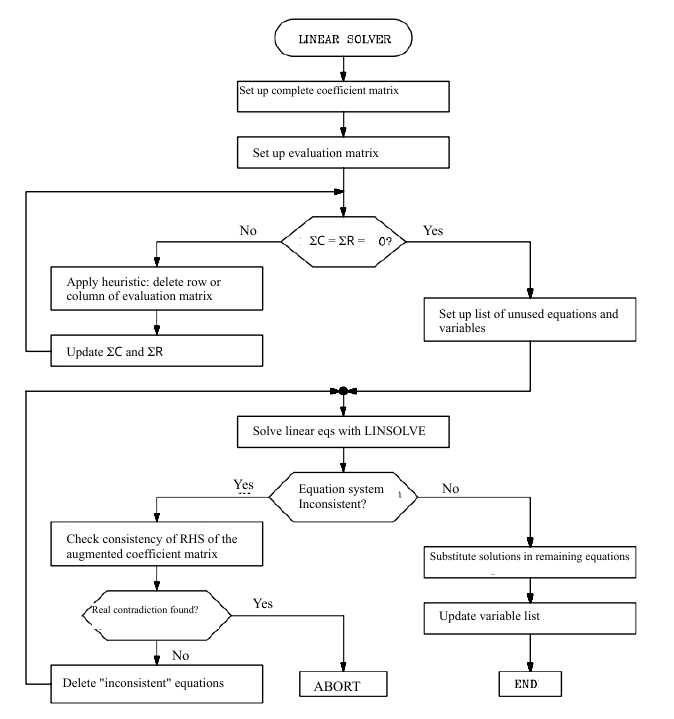
\includegraphics[height=8cm]{LinearEn.png}
\caption \protect {\begin {minipage} [h] {10cm}% --- TABLE
Flow diagram of the Linear Solver\label{AblLinear}
\end {minipage}
}
\end {center}
\end {figure}
%\inbildpsf{Ablaufdiagramm des Linear Solvers}{linear.eps}{160mm}%
%{AblLinear}

\clearpage

\subsection{The Valuation Solver} %%% 2.2.4  =================

The {\em Valuation Solver} first checks,  whether equations and variables still  are available, which can be solved. 
If this is the case, then for the remaining equations two valuation matrices are set up, which serve as basis for the solution sequence order. Both matrices have the dimensions $n \times m$, whereby $n$ is the number of the equations and $m$ the number of variables,  looked for at the moment. The first matrix, the  {\em  path matrix of variables}, contains for each equation the number of  paths for this variable (see section \ref{KomplBewertung})) w.r.t each variable. The second matrix is the  {\em valuation matrix}. Their entries are calculated by the heuristic operator tree valuations of each equation w.r.t. each variable.


To these two matrices one applies  afterwards  -- depending on whether an internal or user-defined  is desired -- an valuation strategy, which arranges the pairs of equation/variables in such a way, that the first items  in this list are the most promising candidates for a following solution attempt  by means of the \verb+SOLVE+ command.

As long as not all proposals for solutions in the list were tried  and no correct solution for one of the suggestions was  calculated, on the basis the determined solution order the next equation from the equation list is selected and tried to solve. If this does not succeed, one or more user-defined transformation functions (if available) for the transformation of the equation are applied and  in each case a solution attemptsare  made.  If these are also without result, the next proposal for a solution is tried.

If  none of the equations is solvable after any variable any more, then the {\em Valuation Solver} returns the unresolved equations in implicit form additionally to all solutions found up to this point, so that these  may be treated later with a numeric procedure. With a successful solution attempt all single solutions (nonlinear equations may have multiple solutions) are checked separately for consistency with the remaining equations. Those solutions, which lead to contradictory predicates, are rejected and with them the corresponding solution path.

If after the consistency check no solution  remains, then the system of equations is inconsistent, and the  {\em Valuation Solver} aborts.  If exactly one solution remains, then this solution is appended to the solution list and substituted into the remaining equations. Finally the list of the wanted variables is updated, whilst the variable just calculated is removed from it and new variables, possibly contained in the solution,  are added. These  can be variables, which are not given as parameters and also not indicated as looked-for. The main solution loop of the {\em Valuation Solvers} begins then again from the start.

With consistent multiple solutions all solution paths must be pursued separately. Fot that the {\em Valuation Solver} calls itself recursively with the remaining equations and variables for each individual solution  and stores the outputted results in a hierarchically structured solution list. Their expansion is task of the {\em Solver Postprocessors} described in the next section.


\clearpage

\begin {figure} [htbp]
\begin {center}
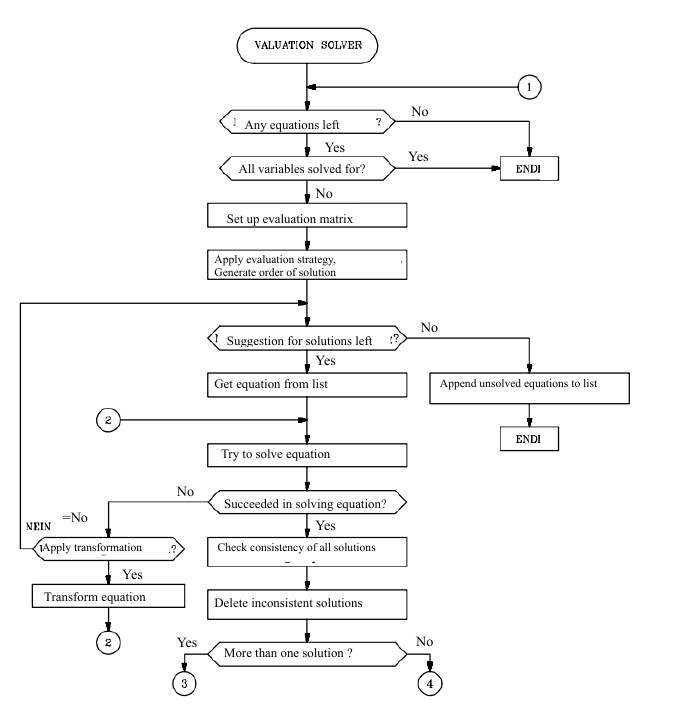
\includegraphics[height=8cm]{Valsolv1En.png}
\caption \protect {\begin {minipage} [h] {10cm}% --- TABLE
Flow diagram of the Valuation Solver (part 1)\label{AblValSolv1}
\end {minipage}
}
\end {center}
\end {figure}

%\inbildpsf{Ablaufdiagramm des Valuation Solvers (Teil 1)}{valsolv1.eps}%
%{157mm}{AblValSolv1}

\clearpage

\begin {figure} [htbp]
\begin {center}
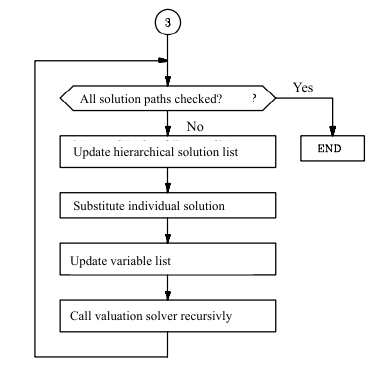
\includegraphics[height=8cm]{Valsolv2aEn.png}
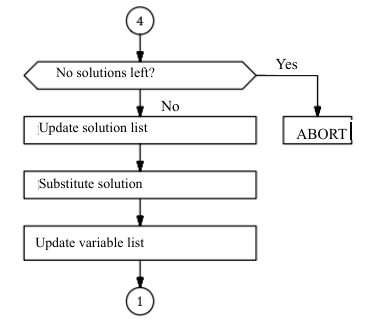
\includegraphics[height=8cm]{Valsolv2bEn.png}
\caption \protect {\begin {minipage} [h] {10cm}% --- TABLE
Flow diagram of the Valuation Solver (part 2)\label{AblValSolv2}
\end {minipage}
}
\end {center}
\end {figure}

%\inbildpsf{Ablaufdiagramm des Valuation Solvers (Teil 2)}{valsolv2.eps}%
%{79mm}{AblValSolv2}

\clearpage


%%% 2.2.4 ====================
\subsection{The Solver Postprocessor}

\begin {figure} [htbp]
\begin {center}
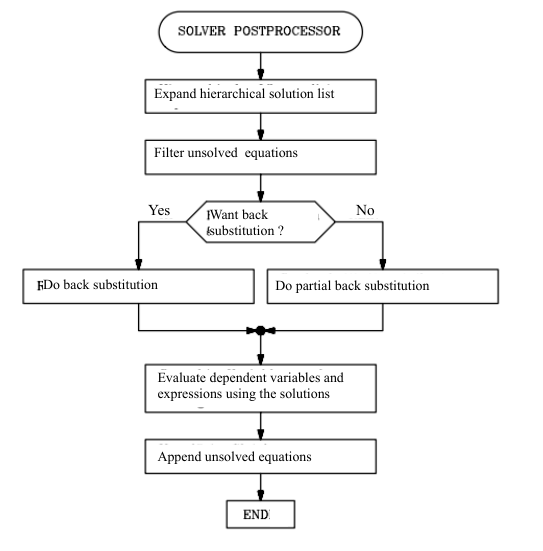
\includegraphics[height=8cm]{PostProcEn.png}
\caption \protect {\begin {minipage} [h] {10cm}% --- TABLE
Flow diagram of the Solver Postprocessor\label{AblPostproc}
\end {minipage}
}
\end {center}
\end {figure}

%\inbildpsf{Ablaufdiagramm des Solver Postprocessors}{postproc.eps}%
%{106mm}{AblPostproc}

The Valuation Solver supplies in the case of multiple solutions of nonlinear equations a hierarchically structured list of results (because of the recursive pursuit of the solution paths) as function value, therefore  the {\em Solver Postprocessor} must dissolve  the list hierarchy at the beginning, so that the back substitution can be executed.

If not all equations within a solution path could be solved  symbolically, then the result list contains the list of the remaining, unresolved nonlinear equations additionally to the variables, for which a solution was found. These will provisionally removed from the equation list and buffered, in order to be added later to the final result.

Depending upon the desire of the user, the back substitution of the system of equations takes place afterwards, which is present up to this point still in upper triangle form. For that, the solution list is evaluated iterative with itself, until no modification of the results is to be seen any  more. Even, if the back substitution is not required by the user\footnote{This requires to set the option variable {\tt SolverBacksubst} to {\tt FALSE} (see section \ref{Optionen})}, it  is nevertheless executed, but only so far as necessary, in order to eliminate all not specified command line variables  from the solutions. If e.g. a system of equations
in the variables $x$, $y$, $z$ and $w$ is to be solved only after the variables $x$ and $y$  and the solution process gives  the triangle form
\begin{eqnarray}
x &=& f_1(y,z,w)\\
y &=& f_2(z,w)  \\
w &=& f_3(z)    \\
z &=& \const,
\end{eqnarray}
so the complete back substitution leads to the result
\begin{eqnarray}
x &=& \const \\
y &=& \const
\end{eqnarray}
With switched off complete back substitution, the following two equations are given back 
\begin{eqnarray}
x &=& g(y) \\
y &=& \const
\end{eqnarray}
which does not contain the internal variables $z$ und $w$ any longer, but are further coupled by the variable $y$ among themselves.

After termination of the back substitution and the evaluation of the composite terms in the variable list of the command line using the solutions, the at first filtered unresolved equations are again appended to the solution list. The finished solution list is then given to the user as function value.


\section{Application of {\tt Solver}}  % ch. 2.3

\subsection{Command syntax}

The call of  {\tt Solver} from the Maxima command line use the syntax

\begin{literatim}{|}
    Solver( list_of_equations, list_of_variables, list_of_parameters )
\end{literatim}
or, if the system of equations, which is to be solved, does not contain any parameters, also with
\begin{literatim}{|}
    Solver( list_of_equations, list_of_variables )
\end{literatim}
The list of   equations is a list of Maxima objects, for which \verb+EquationP+ equals \verb+TRUE+. The system of equations
(\ref{linearxyz}) -- (\ref{linearxy}) is thus formulated in the following way:
\begin{literatim}{|}
(COM5) Equations :
[
    x + 2*y -     z =  6,
  2*x + y*z -   z^2 = -1,
  3*x -   y + 2*z^2 =  3
]$
\end{literatim}
The unknown variables are told to the Solver likewise in form of a list, e.g. as
\begin{literatim}{|}
     [x, y, z]
\end{literatim}
for the above-mentioned systen of equations. Beside purely atomic variable symbols  (\verb+SymbolP+) the variable list may contain  also composite terms in the looked-for unknowns. If for the system of equations  the variables $x$, $y$ 
and $z$ are not explicitly searched, but rather $x$ and the value  $\sin(\pi yz)$, then the variable list reads
\begin{literatim}{|}
     [x, sin(%pi*y*z)] .
\end{literatim}

The parameter list must contain exclusively atomic symbols, thus only objects with  \verb+SymbolP+ equals \verb+TRUE+. 
Composite terms are here neither admissible nor meaningfully.

\subsection{Special Features of the Syntax of Equations}

At this point we refer to some differences of the command syntax in  comparison with the admissible invocations of the Maxima build-in \verb+SOLVE+ function. The latter may also get the equations in {\em Expression} form, i.e. as expressions  $\verb#EquationP# = \verb#FALSE#$, which are implicitly understood  as equations of the form $\mbox{\em Expression} = 0$:
\begin{literatim}{|}
     [
         x + 2*y -     z - 6,  \$\leftarrow\$ {\rm{}not  admissable}
       2*x + y*z -   z^2 + 1,
       3*x -   y + 2*z^2 - 3
     ]$
\end{literatim}
This form of representation of the equation  is used internally, e.g. by the {\em 
Valuation Solver}, but is not permitted as call of the Solver in the command line. Furthermore, the \verb+SOLVE+ function permits  omitting the brackets around the arguments, if only one equation and/or only one variable is to be transferred. This is  also not admissible with the use of Solver.

\subsection{Example Calls of Solver}

\begin{example}{SolverExample1}
For the input of the system of equations \verb+COM5+  a correct call of the Solver is the instruction in the command line \verb+COM7+. 
The specification of the calculated solutions is done in form of a list of solution lists, see output line \verb+D7+.
\begin{literatim}{|}
(COM6) MsgLevel : 'DETAIL$   {\rm/* see section \ref{Optionen} */}

(COM7) Solver( Equations, [x, y, z] );

{\rm{}Output of}{\em Solver Preprocessors}{\rm:}
The variables to be solved for are [X, Y, Z]
Checking for inconsistencies...
... none found.

{\rm{}Output of}{\em Immediate Assignment Solvers}{\rm:}
Searching for immediate assignments.
No immediate assignments found.

{\rm{}Output of}{\em Linear Solvers}{\rm:}
Searching for linear equations...
  ...with respect to: [X, Y, Z]
Found 2 linear equations in 2 variables.
The variables to be solved for are [X, Y]
                                         2
The equations are [- Z + 2 Y + X - 6, 2 Z  - Y + 3 X - 3]
Solving linear equations.
                            2                  2
                         4 Z  - Z - 12      2 Z  + 3 Z + 15
The solutions are [X = - -------------, Y = ---------------]
                               7                   7
Searching for linear equations...
  ...with respect to: [Z]
No linear equations found.

{\rm{}Output of}{\em Valuation Solvers}{\rm:}
Checking for remaining equations.
1 equation(s) and 1 variable(s) left.
The variables to be solved for are [Z]
Trying to solve equation 1 for Z

{\rm{}Here  a complexity valuation Is not needed,}
{\rm{}because there is only one equation and one variable left.}
Valuation: (irrelevant)
                   3       2
The equation is 2 Z  - 12 Z  + 17 Z + 31 = 0
Checking if equation was solved correctly.
                         SQRT(13) %I - 7      SQRT(13) %I + 7
The solutions are [Z = - ---------------, Z = ---------------, Z = - 1]
                                2                    2
Solution is correct.

{\rm{}Individual consistency check w.r.t. multiple solutions:}
The solution is not unique. Tracing paths separately.
Solution 1 for Z
Checking for inconsistencies...
... none found.
Solution 2 for Z
Checking for inconsistencies...
... none found.
Solution 3 for Z
Checking for inconsistencies...
... none found.
                                    SQRT(13) %I - 7      SQRT(13) %I + 7
Consistent solutions for Z : [Z = - ---------------, Z = ---------------,
                                           2                    2

                                                                   Z = - 1]

{\rm{}Recursive pursuit of all three solution paths:}
Checking for remaining equations.
All variables solved for. No equations left.
Checking for remaining equations.
All variables solved for. No equations left.
Checking for remaining equations.
All variables solved for. No equations left.

{\rm{}Output of}{\em Solver Postprocessors}{\rm:}
Postprocessing results.

            27 SQRT(13) %I - 41        17 SQRT(13) %I - 87
(D7) [[X = -------------------, Y = - -------------------,
                    14                         14

      SQRT(13) %I - 7          27 SQRT(13) %I + 41      17 SQRT(13) %I + 87
Z = - ---------------], [X = - -------------------, Y = -------------------,
             2                         14                       14

    SQRT(13) %I + 7
Z = ---------------], [X = 1, Y = 2, Z = - 1]]
           2
\end{literatim}
For an better overview, here is the result again in TEX-output:
\begin{equation}
\left[
   x = {{27\,\sqrt{13}\,i-41}\over{14}},  \,\,
   y = -{{17\,\sqrt{13}\,i-87}\over{14}}, \,\,
   z = -{{\sqrt{13}\,i-7}\over{2}}
\right]
\end{equation}
\begin{equation}
\left[
   x = -{{27\,\sqrt{13}\,i+41}\over{14}}, \,\,
   y = {{17\,\sqrt{13}\,i+87}\over{14}}, \,\,
   z = {{\sqrt{13}\,i+7}\over{2}}
\right]
\end{equation}
\begin{equation}
\left[
   x =  1, \,\,
   y =  2, \,\,
   z = -1 
\right]
\end{equation}
\end{example}

\begin{example}{SolverExample2}
As  second example, the following system of equations parameterized in $a$ and $b$
\begin{eqnarray}
3ax + y^2 &=& 1 \\
 bx - y   &=& -1
\end{eqnarray}
is to be solved for the variables $x$ and $y$ as well as the composite term $x/y$ . Since the system of equations does not contain any direct assignments and in this case a repeated search for linear equations  is not meaningful, the {\em Immediate Assignment Solver} and the repetition loop of the {\em Linear Solvers}  are switched off with the instruction \verb+COM8+:
\begin{literatim}{|}
(COM8) SolverImmedAssign : SolverRepeatLinear : FALSE$

(COM9) ParEq : [ 3*a*x + y^2 =  1, b*x - y = -1 ]$

(COM10) Solver( ParEq, [x, y, x/y], [a, b] );

                                       X
The variables to be solved for are [X, -, Y]
                                       Y
The parameters are [A, B]
Checking for inconsistencies...
... none found.
Trying to solve for [X, Y]
                                     X
in order to solve for the expression -
                                     Y
Searching for linear equations...
  ...with respect to: [X, Y]
Found 1 linear equations in 2 variables.
The variables to be solved for are [X, Y]
The equations are [- Y + B X + 1]
Solving linear equations.
The solutions are [Y = B X + 1]

Checking for remaining equations.
1 equation(s) and 1 variable(s) left.
The variables to be solved for are [X]
Trying to solve equation 1 for X
Valuation: (irrelevant)
                 2  2
The equation is B  X  + (2 B + 3 A) X = 0
Checking if equation was solved correctly.
                         2 B + 3 A
The solutions are [X = - ---------, X = 0]
                             2
                            B
Solution is correct.
The solution is not unique. Tracing paths separately.
Solution 1 for X
Checking for inconsistencies...
... none found.
Solution 2 for X
Checking for inconsistencies...
... none found.
                                    2 B + 3 A
Consistent solutions for X : [X = - ---------, X = 0]
                                        2
                                       B
Checking for remaining equations.
All variables solved for. No equations left.
Checking for remaining equations.
All variables solved for. No equations left.
Postprocessing results.

              2 B + 3 A        B + 3 A  X   2 B + 3 A                   X
(D10) [[X = - ---------, Y = - -------, - = ----------], [X = 0, Y = 1, - = 0]]
                  2               B     Y    2                          Y
                 B                          B  + 3 A B
\end{literatim}
\end{example}





\section{\label{Optionen}The Options of {\tt Solver}}  % 2.4 ====================================
 
Using  the Maxima command line (\verb+Macsyma toplevel+) or a program file, the behavior of the Solver can be influenced by the individual setting of a set of option variables, which are listed and described in the following. Behind the names of the option variables, the standard assignments (values/symbols) are given  in angle parentheses, which are set automatically on the first start of the module \verb+SOLVER+.

\begin{description}

\item[{\tt MsgLevel <SHORT>}] ({\em message level}) 
controls the scope of the displayed messages during the program run. The assignments \verb+OFF+, \verb+SHORT+ and
\verb+DETAIL+ are admissible. 
\nl
Becomes  \verb+MsgLevel : OFF+, then all program outputs are completely suppressed. In the case of  \verb+SHORT+ only status informations are returned whilst the program is running. The keyword \verb+DETAIL+  causes additionally the output of all of the Solver modules intermediate results and also of messages of the decisions made due to the heuristics.
%
%
\item[{\tt SolverImmedAssign <TRUE>}] 
switches the {\em Immediate 
Assignment Solver} on (\verb+TRUE+) resp.\ off (\verb+FALSE+). If the module is switched on, then before the call of {\em Linear Solvers} the system of equations is searched for direct allocations of the form $\mbox{\em 
var} = \const$ or $\const = \mbox{\em var}$, which can be inserted immediately into the remaining equations.
%
%
\item[{\tt SolverRepeatImmed <TRUE>}] 
determines whether the {\em Immediate 
Assignment Solver}  is called repeatedly (\verb+TRUE+), until no more direct assignments are found, or whether only one call takes place  (\verb+FALSE+).
%
\item[{\tt SolverSubstPowers <FALSE>}] ({\em substitute powers})
controls the handling of variables, which occur in powers $p_k$
of integer multiples $p_k=k p_0$, $k \in \nz$, of a basic power $p_0
\in \nz \setminus \{ 1 \}$.
If the system of equations contains e.g. the variable  $x$ exclusively in the powers $x^2$, $x^4$,
$x^6$, \ldots, e.g. $p_0=2$, then  by \verb+SolverSubstPowers:TRUE+ the term $x^{p_0}=x^2$ is substituted with the
new variable symbol $X2$, that therfore only occurs in the powers $X2$, $X2^2$, $X2^3$, \ldots. 
In this way the degree of the equations which are to be solved is reduced as well as the solution variety. 
However, if necessary, a rework of the solutions are necessary.
%

\item[{\tt SolverInconsParams <ASK>}] ({\em inconsistent parameter handling}) 
influence the behavior of the routine for the consistency check. Admissible parameters are \verb+ASK+, \verb+BREAK+
and \verb+IGNORE+.
If  during the consistency  check a dependency between the  parameters is discovered, then with \verb+SolverInconsParams : ASK+ the users is asked for the validity of the appropriate constrained condition.  With a positive response, this is stored  for later evalutaion in the list  \verb+SolverAssumptions+. If the dependency is not admissible or if the option variable is set with \verb+BREAK+, then the solution process is aborted. If the parameter is set to \verb+IGNORE+,  then the consistency check is caused to accept basically all constrained conditions between parameters as valid as long as these do not contradict directly already made conditions.
%
\item[{\tt SolverLinear <TRUE>}] 
switches the {\em Linear Solver} on
(\verb+TRUE+) resp.\ off (\verb+FALSE+). Switching off is recommended if the system of equations, which is to be solved, does not contain linear equations or their number is very small in relation to the number of  nonlinear equations. In these cases much computing time can be saved through bypass the {\em Linear Solvers}, since the algorithm to search for linear equations is quite complex.
%
\item[{\tt SolverRepeatLinear <TRUE>}] 
cause repeated calls of {\em Linear Solvers}. If the variable is set to \verb+FALSE+, then  {\em Linear Solver} is executed only once.
%
\item[{\tt SolverFindAllLinearVars <TRUE>}] 
decides whether  {\em 
Linear Solver}  that looks for maximal large  pieces of linear equations regarding all available variables (\verb+TRUE+), or whether only subsystems in the variables are to be extracted, which are immediately looked for during the solution process (\verb+FALSE+). The setting of the variables plays especially a role, if under-determined systems of equations are to be solved. 
\nl Here \verb+SolverFindAllLinearVars : FALSE+ should to be set, because otherwise no solutions for the originally interesting variables could possibly be found due to the too small number of equations. With \verb+FALSE+ it is guaranteed that at first after these variables is solved and the degrees of freedom are expressed in the other unknowns.
%
\item[{\tt SolverValuationStrategy <MinVarPathsFirst>}] 
 contains the name of the function, which is generate a solution order from the variable path matrix and the valuation matrix   (see section \ref{SolverValuationStrategies}). The call of the function within the {\em Valuation Solvers} is done with:
des {\em Valuation Solvers} mit:
\begin{literatim}{|}
     SolveOrder : Apply( 
       SolverValuationStrategy, [ VarPathMatrix, ValuationMatrix ]
     )
\end{literatim}
As function value a list of the form
\begin{literatim}{|}
     [ [i1, j1, b1], [i2, j2, b2], ... ]
\end{literatim}
 is expected, which was  
 described in section  \ref{KomplBewertung}. \nl To observe here is the option variable \verb+SolverMaxLenValOrder+.
%
\item[{\tt SolverDefaultValuation <10>}] 
determines the valuation factor for operators, which were not explicitly assigned such a factor with the \verb+SetProp+ instruction  (see section \ref{ChgOpValuations}).
%
\item[{\tt SolverMaxLenValOrder <5>}] ({\em maximum length of valuation order}) 
determines the maximal length of the solution order. If the last proposal for solution in the list does not lead to success, then the  {\em Valuation Solver} aborts the solution process, even if not all pairs of equation/variables were tried.
%
\item[{\tt SolverTransforms <[]>+}] 
contains a list of the names of functions, which can be applied after a unsuccessful solution attempt to the corresponding equation, in order to increase the solution chances with a renewed attempt. Thereby the functions are executed  in the order of their occurring in the list. After each function call  the next solution attempt takes place directly. If this fails, then the next transformation in the list is applied, as long as the equation could be solved or no further transformation is available. Since the possibilities for manipulations  with the transformations are quite extensive,  a more accurate specification of their definition and application is in section \ref{SolverTransforms}.
%
\item[{\tt SolverPostprocess <TRUE>}] 

switches the {\em Solver 
Postprocessor}  on (\verb+TRUE+) resp.\ off (\verb+FALSE+).  If switched to status off,  the hierarchical result list of the Solver is returned without rework, e.g. without expansion, back substitution and extraction of the variables requested by the user. This control variable serves primarily for Debug purposes.
%
\item[{\tt SolverBacksubst <TRUE>}] ({\em backsubstitution}) 
determines whether the {\em Solver Postprocessor}  is to execute a back substitution of the system of equations brought on triangle form (\verb+TRUE+) or not (\verb+FALSE+). If the calculated symbolic solutions are very extensive, then it is often meaningful to execute no complete back substitution, but to output some of the looked-for variables as functions of other calculated unknowns.
%
\item[{\tt SolverDispAllSols <FALSE>}] ({\em display all solutions}) 
instructs the Solver, if set to \verb+TRUE+,  to output {\em all} found solutions at the termination of the solution process  and not only for the variables indicated by the user.
%
\item[{\tt SolverRatSimpSols <TRUE>}] ({\em perform rational simplifications on solutions}) 
instructs the {\em Solver Postprocessor}  to simplify the results  with the instruction \verb+FullRatSimp+ before the output.
%
\item[{\tt SolverDumpToFile <FALSE>}] 
 (\verb+TRUE+) instructs the {\em Valuation Solver},  to write all found solutions (after each successful solution attempt) as well as the remaining equations and variables into a Maxima batch file, whose name is saved in the option variable  \verb+SolverDumpFile+. This option is intended for extensive problems, where Maxima is inclined  to system crashes because of  acute lack of main and swap memory.
Within a crash,  at least a part of the results can be saved by the storage of the intermediate results.
%

\item[{\tt SolverDumpFile <"{}SOLVER.DMP"{}>}] 
contains the name of the file, into which the intermediate results are to be written.

\end{description}


% -----------------------------------------------------------------------------
%\stop  %%% STOPPED here with translation, wL 20.11.23
% -----------------------------------------------------------------------------


\section[user specific transformation routines]{Definition and
Integration of User Specific Transformation Routines\label{SolverTransforms}} %==================== 2.5

Often the {\em Valuation Solver} encounters equations during the solution process, which it is not able to solve, although already some simple rearrangements or simplifications could help, in order to receive the desired result. E.g.\  the \verb+SOLVE+ function is not able to solve the equation
\begin{equation}
x + \sin^2 x + \cos ^2 x = 1
\end{equation}

correctly for $x$, since it does not know that the square terms of sine and cosine  can be combined easyly into '1'.

In order to be able to execute rearrangements or simplifications of the equations depending upon the application case, the dynamic integration of user-defined transformation functions is bulid in the Solver, which are applied to unresolved equations if necessary. The  {\em Valuation
Solver}  transfers to these functions among other things the equation and the variable, after which the equation is to be solve. The transformation function has now the task to transform the equation and return it as its function value again to the Solver, so that a renewed solution attempt can begin.

The call of a transformation function from the Solver works in the following way:

\begin{literatim}{|}
     Transform : CopyList( SolverTransforms ),
       \vdots
     SOLVER LOOP
          \vdots
        Trans : Pop( Transform ),
        TransEq : Apply( Trans, [ Equation, Variable, Solution ] )
          \vdots
     LOOP END
\end{literatim}

Thereby  the additionally transferred parameter \verb+Solution+ contains the result of the failed solution attempt, on the basis of which possibly helpful conclusions can be drawn. The following instruction shows an example of the definition of a simple, user specific transformation routine, which tries to make an equation solvable by simplifying of trigonometric functions:
\begin{literatim}{|}
     TransformTrig( Equation, Variable, Solution ) := 
       TrigSimp( Equation )$
\end{literatim}

For the integration of the function  their name had to be inserted into the \nl global list \verb+SolverTransforms+:
\begin{literatim}{|}
     SolverTransforms : [ 'TransformTrig ]$
\end{literatim}


Also the application of a transformation routine may  be unsuccessful, therefore it exists the possibility to remember the Solver the failure of the simplifying attempt by return of an empty list (\verb+[]+) as function value. In this way it is prevented that a further call of the
\verb+SOLVE+ function with the same equation takes place. Instead the Solver tries directly,  to execute the next transformation in the list, if available,.
For an alternative to the rearranging of the equation and an afterward solution by the {\em internal} Solver, a transformation routine is also allowed, to determine the solutions of the transferred equation  {\em itself} and return them in the form
\begin{literatim}{|}
     [ Variable = Solution_1, Variable = Solution_2, ... ] 
\end{literatim}

A possible area of application for such functions would be the application of numeric procedures for the solution of nonlinear equations, which  contain only  one variable and no parameters. Or the equation can be manipulated by hand, 
whilst  the transformation routine calls a   {\em Maxima-Break}. 
The method for the definition and integration of transformation functions with success return, wil be demonstrated in the following completely worked example. To solve is the system of equations (\ref{Trig1}) --  (\ref{Trig3})  for the variables  $x$, $y$
and $z$. This task is quite simple in principle, but nevertheless it causes substantial difficulties  to the Solver.
\begin{eqnarray}
        z - \sin x &=& 0 \label{Trig1} \\
y + z^2 + \cos x^2 &=& 5               \\
             y + x &=& 1 \label{Trig3}
\end{eqnarray}

At first, the system of equations is input as an equation list as well as the variables:
\begin{literatim}{|}
(COM11) TrigEq :
[
          z - sin(x) = 0,
  y + z^2 + cos(x)^2 = 5,
               y + x = 1
]$

(COM12) Var : [x, y, z]$
\end{literatim}

The first solution attempt is to be executed without transformation functions:

\begin{literatim}{|}
(COM13) SolverTransforms : []$

(COM14) Solver( TrigEq, Var );

The variables to be solved for are [X, Y, Z]
Checking for inconsistencies...
... none found.

Searching for linear equations...
  ...with respect to: [X, Y, Z]
Found 2 linear equations in 2 variables.
The variables to be solved for are [Y, Z]
The equations are [Z - SIN(X), Y + X - 1]
Solving linear equations.
The solutions are [Y = 1 - X, Z = SIN(X)]

Checking for remaining equations.
1 equation(s) and 1 variable(s) left.
The variables to be solved for are [X]
Trying to solve equation 1 for X
Valuation: (irrelevant)
                   2         2
The equation is SIN (X) + COS (X) - X - 4 = 0
Checking if equation was solved correctly.
                          2         2
The solutions are [X = SIN (X) + COS (X) - 4]
Solution is not correct.
Cannot solve equation. Giving up.

Postprocessing results.
Cannot determine an explicit solution for X

                                          2         2
(D14)        [[Y = 1 - X, Z = SIN(X), [SIN (X) + COS (X) - X - 4]]]
\end{literatim}

In this case the Solver is not able to solve the equation with the squared sine and cosine terms for the variable $x$ and therefore returns  the unresolved equation in implicit form as last item of the solution list. 
To simplifyf the equations two transformation functions are now to be defined and merged in. The first transformation serves for the simplification of logarithm terms, the second for the simplification of terms, which contain trigonometric functions. Both functions check whether their application was successful and returns an empty list, if the transformation did not cause any modification of the equation.
\begin{literatim}{|}
(COM15) TransformLog( Equation, Variable, Solution ) := BLOCK(
  [ Eq ],
  Eq : LogContract( Equation ),
  IF Eq = Equation THEN
    RETURN( [] )
  ELSE
    RETURN( Eq )
)$

(COM16) TransformTrig( Equation, Variable, Solution ) := BLOCK(
  [ Eq ],
  Eq : TrigSimp( Equation ),
  IF Eq = Equation THEN
    RETURN( [] )
  ELSE
    RETURN( Eq )
)$
\end{literatim} 

The transformation function \verb+TransformLog+ may be applied basically as first, therefore the integration of the routines takes place in the following order:

\begin{literatim}{|}
(COM17) SolverTransforms : [ 'TransformLog, 'TransformTrig ]$
\end{literatim}
Now a new run of Solver may be started.
\begin{literatim}{|}
(COM18) Solver( TrigEq, Var );

The variables to be solved for are [X, Y, Z]
Checking for inconsistencies...
... none found.

Searching for linear equations...
  ...with respect to: [X, Y, Z]
Found 2 linear equations in 2 variables.
The variables to be solved for are [Y, Z]
The equations are [Z - SIN(X), Y + X - 1]
Solving linear equations.
The solutions are [Y = 1 - X, Z = SIN(X)]

Checking for remaining equations.
1 equation(s) and 1 variable(s) left.
The variables to be solved for are [X]
Trying to solve equation 1 for X
Valuation: (irrelevant)
The equation is SIN (X) + COS (X) - X - 4 = 0
Checking if equation was solved correctly.
                          2         2
The solutions are [X = SIN (X) + COS (X) - 4]
Solution is not correct.
\end{literatim}

Here the Solver recognize as in the preceded case that it cannot solve the equation and applies the first transformation in the list to it.
\begin{literatim}{|}
Applying transformation TRANSFORMLOG
Transformation failed.
\end{literatim}

Since the equation does not contain logarithmic functions, the simplifying attempt is not successful. Therefore the second transformation routine is tried.
\begin{literatim}{|}
Applying transformation TRANSFORMTRIG
The transformation yields - X - 3 = 0
Retrying with transformed equation.
Checking if equation was solved correctly.
The solutions are [X = - 3]
Solution is correct.

Solution 1 for X
Checking for inconsistencies...
... none found.
Consistent solutions for X : [X = - 3]
Checking for remaining equations.
All variables solved for. No equations left.
Postprocessing results.

(D18)                   [[X = - 3, Y = 4, Z = - SIN(3)]]
\end{literatim}

The transformation function \verb+TransformTrig+ succeeds to simplfy the equation, so that the Solver is now able, to determine the correct solution for the variable $x$.







\section{Modification of the Operator Valuations\label{ChgOpValuations}}  % ch 2.6 =====================

To give the user of the Solver the possibility for an individual intervention of the heuristic complexity valuation of algebraic terms,  the valuations of the arithmetic operators are stored as {\em Macsyma Properties}  under the keyword \verb+Valuation+, and not as immutable constants. The definition of a valuation factor takes place with the instruction

\begin{literatim}{|}
     SetProp( {\em{}Operator}, 'Valuation, {\em{}Valuation factor} )$
\end{literatim}

The standard mappings of the valuation factors are pre-defined in the Solver:
\begin{literatim}{|}
     SetProp( 'sin,   'Valuation, 10 )$
     SetProp( 'cos,   'Valuation, 10 )$
     SetProp( 'tan,   'Valuation, 10 )$
     SetProp( 'asin,  'Valuation, 12 )$
     SetProp( 'acos,  'Valuation, 12 )$
     SetProp( 'atan,  'Valuation, 12 )$
     SetProp( 'sinh,  'Valuation, 12 )$
     SetProp( 'cosh,  'Valuation, 12 )$
     SetProp( 'tanh,  'Valuation, 12 )$
     SetProp( 'asinh, 'Valuation, 12 )$
     SetProp( 'acosh, 'Valuation, 12 )$
     SetProp( 'atanh, 'Valuation, 12 )$
     SetProp( "{}+"{},    'Valuation,  1 )$
     SetProp( "{}-"{},    'Valuation,  1 )$
     SetProp( "{}*"{},    'Valuation,  4 )$
     SetProp( "{}/"{},    'Valuation,  4 )$
     SetProp( "{}^"{},    'Valuation, 10 )$
     SetProp( 'exp,   'Valuation, 10 )$
     SetProp( 'log,   'Valuation, 10 )$
     SetProp( 'sqrt,  'Valuation, 10 )$
\end{literatim}

E.g. if the valuation of the tanh--operator should be modified on 20, then this can be done at any time by
\begin{literatim}{|}
     SetProp( 'tanh, 'Valuation, 20 )$
\end{literatim}

A quality factor can queried with the \verb+Get+ command:
\begin{literatim}{|}
     Get( {\em{}Operator}, 'Valuation );
\end{literatim}
Example: The valuation of ``$*$''-- operator is determined through:

\begin{literatim}{|}
(COM19) Get( "{}*"{}, 'Valuation );

(D19)                                   4
\end{literatim}

If the result of the query has  the value \verb+FALSE+,  then this means that no valuation factor for the operator concerned was defined.




\section[User Specific Valuation Strategie]% ch 2.7 ===============================================
{Definition and Integration of \\User Specific Valuation Strategies%
\label{SolverValuationStrategies}}

By means of a reassignment of the procedure variable \verb+SolverValuationStrategy+ the {\em Valuation Solver} is caused to use  a user-defined valuation strategy to the determination of the solution order instead of the internal function. The function are given by their call 
two valuation matrices,
\begin{literatim}{|}
     SolveOrder : Apply(
       SolverValuationStrategy, [ VarPathMatrix, ValuationMatrix ]
     )
\end{literatim}
which are the  {\em variable path matrix} and the {\em complexity valuation matrix}, whose row dimension equal the number of the equations and their column dimension equals the number of variables which are be determined.

The entry at the position $(i,j)$ of the {\em variable path matrix} corresponds to the number of paths to the instances of the variable $x_j$ in equation  $i$ (see section \ref{KomplBewertung}). The {\em complexity evaluation matrix} contains at the position $(i,j)$ the complexity valuation of the equation $i$
w.r.t. the variable $x_j$. Thus, for the system of equations (\ref{linearxyz}) -- (\ref{linearxy})
the path matrix reads 

$$
\bordermatrix{
                  & x & y & z \cr
(\ref{linearxyz}) & 1 & 1 & 1 \cr 
(\ref{linearx})  & 1 & 1 & 2 \cr 
(\ref{linearxy}) & 1 & 1 & 1 \cr 
}
$$

%\begin{displaymath}
%\bordermatrixlr{\left[}{
%                  & x & y & z \cr
% & 1 & 1 & 1 \cr %(\ref{linearxyz})
%  & 1 & 1 & 2 \cr %(\ref{linearx}) 
% & 1 & 1 & 1 \cr %(\ref{linearxy}) 
%}{\right]}
%\end{displaymath}
and the valuation matrix using the standard operator valuation factors are determined to

\begin{displaymath}
\bordermatrix{
                  & x & y &  z \cr
(\ref{linearxyz}) & 1 & 4 &  1 \cr
(\ref{linearx})   & 4 & 4 & 14 \cr
(\ref{linearxy})  & 4 & 1 & 40 \cr
}
\end{displaymath}

%\begin{displaymath}
%\bordermatrixlr{\left[}{
%                  & x & y &  z \cr
%(\ref{linearxyz}) & 1 & 4 &  1 \cr
%(\ref{linearx})   & 4 & 4 & 14 \cr
%(\ref{linearxy})  & 4 & 1 & 40 \cr
%}{\right]}
%\end{displaymath}

\noindent
From these matrices the valuation strategy must generate  a solution order (see section \ref{KomplBewertung})) in the form

\begin{literatim}{|}
     [ [i1, j1, b1], [i2, j2, b2], ...  ]
\end{literatim}
The maximal length of the list should not be larger than the value of the option variable \verb+SolverMaxLenValOrder+.

The basic structure of an valuation strategy is given by the following pseudocode:

\begin{literatim}{|}
     MyValuationStrategy( PathMat, ValMat ) := BLOCK(
       
       {\rm{}generate a solution order from the valuation strategies} 
       {\rm{}limit the length of the list to} SolverMaxLenValOrder  {\rm{}elements}

       RETURN( {\rm{}the solution order} )
     )$
\end{literatim}

\noindent
To insert the function afterwards, the procedure variable \verb+SolverValuationStrategy+ is to assign with the function name:

\begin{literatim}{|}
     SolverValuationStrategy : 'MyValuationStrategy$
\end{literatim}
